% begin module improper-integral-type2
\begin{frame}
\frametitle{Type II: Discontinuous Integrands}
We can use the same approach if the function $f$ is discontinuous at one of the endpoints $a$ and $b$ in the integral $\int_a^b f(x) \diff x$.

For example, $\frac{1}{\sqrt{x - 2}}$ is discontinuous at $2$, so we might wonder if the integral
\[
\int_2^5 \frac{1}{\sqrt{x-2}}\diff x
\]
exists.

\begin{center}
\psset{xunit=1cm, yunit=1cm}
\begin{pspicture}(-0.5, -0.5)(5.600000,3.3) 
\psframe*[linecolor=white](-0.5,-0.5)(5.600000,3.3) 
\tiny 
\pscustom*[linecolor=\psColorAreaUnderGraph]{
%Function formula: \frac{1}{(x-2)^{1/2}} 
\psplot[linecolor=\psColorGraph, plotpoints=1000]{2.100000}{5.000000}{1.0000000 -2.0000000 x add 0.5000000 exp div }
\psline(5.000000, 0)(2.00000, 0)(2,3.16227766)
}
%Function formula: \frac{1}{(x-2)^{1/2}} 
\psplot[linecolor=\psColorGraph, plotpoints=1000]{2.100000}{5.000000}{1.0000000 -2.0000000 x add 0.5000000 exp div }

\psaxes[arrows=<->](0,0)(-0.500000,-0.5)(5.5,3.2)
\psLabels{5.5}{3.2}
\end{pspicture} 
%\ 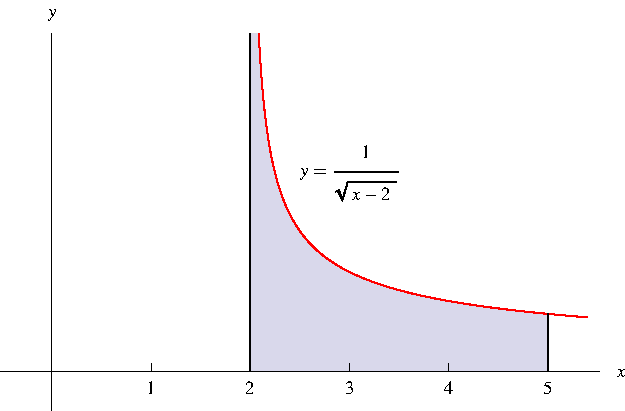
\includegraphics[height=3cm]{improper-integrals/pictures/08-08-ex5.pdf}%
\end{center}
\end{frame}

\begin{frame}
\begin{definition}[Improper Integral of Type II]
\begin{enumerate}
\item  If $f$ is continuous on $[a, b)$ and discontinuous at $b$, then
\abovedisplayskip=0pt
\belowdisplayskip=0pt
\[
\int_a^b f(x) \diff x = \lim_{t\rightarrow b^-} \int_a^t f(x) \diff x
\]
if the limit exists.
\item  If $f$ is continuous on $(a, b]$ and discontinuous at $a$, then
\abovedisplayskip=0pt
\belowdisplayskip=0pt
\[
\int_a^b f(x) \diff x = \lim_{t\rightarrow a^+} \int_t^b f(x) \diff x
\]
if the limit exists.
\end{enumerate}
$\int_a^bf(x) \diff x$ is called convergent if the corresponding limit exists and divergent if it doesn't exist.
\begin{enumerate}
\setcounter{enumi}{2}
\item  If $f$ has a discontinuity at $c$, where $a < c < b$, and both $\int_a^c f(x)\diff x$ and $\int_c^b f(x)\diff x$ are convergent, then we define 
\abovedisplayskip=0pt
\belowdisplayskip=0pt
\[
\int_a^b f(x) \diff x = \int_a^c f(x)\diff x + \int_c^b f(x) \diff x
\]
\end{enumerate}
\end{definition}
\end{frame}
% end module improper-integral-type2
